\documentclass[5p,times]{elsarticle}
\usepackage[T1]{fontenc}
\usepackage{fontspec,etoolbox}
\setmainfont{Times New Roman}
\setsansfont{Arial}
\AtBeginEnvironment{tabular}{\sffamily}
\usepackage{amsmath,amssymb,booktabs,array,graphicx,url,xcolor,placeins,ragged2e}
\usepackage[hidelinks]{hyperref}
\setlength{\emergencystretch}{3em}
\setcounter{topnumber}{3}\setcounter{dbltopnumber}{3}\setcounter{totalnumber}{6}
\renewcommand{\topfraction}{.92}\renewcommand{\dbltopfraction}{.92}
\renewcommand{\textfraction}{.06}\renewcommand{\floatpagefraction}{.8}\renewcommand{\dblfloatpagefraction}{.8}
\graphicspath{{figures/}}
\journal{Aerospace Science and Technology}
\newcommand{\R}{\mathbb{R}}\newcommand{\SO}{\mathrm{SO}(3)}
\newcommand{\norm}[1]{\left\lVert#1\right\rVert}
\newcommand{\sk}[1]{\left[#1\right]_{\times}}
\newcommand{\doi}[1]{\href{https://doi.org/#1}{doi:\nolinkurl{#1}}}
\makeatletter
\def\ps@pprintTitle{\let\@oddhead\@empty\let\@evenhead\@empty
\def\@oddfoot{\hfil\footnotesize\thepage\hfil}\let\@evenfoot\@oddfoot}
\makeatother
\begin{document}
\begin{frontmatter}
\title{Vision- and Tension-Informed Inertial Identification and Formation Reconfiguration for Cooperative Aerial Transport Through Obstacles}
\author[a]{Fangwei Peng}
\author[b]{Juntong Qi\corref{corresponding}}
\ead{qijt@shu.edu.cn}
\author[b]{Yan Peng}
\author[c]{Mingming Wang}
\author[d]{Chong Wu}
\cortext[corresponding]{Corresponding author.}
\address[a]{School of Mechatronic Engineering and Automation, Shanghai University, Shanghai 200444, China}
\address[b]{School of Future Technology, Shanghai University, Shanghai 200444, China}
\address[c]{School of Electrical and Information Engineering, Tianjin University, Tianjin 300072, China}
\address[d]{EFY Intelligent Control (Tianjin) Technology Group Co., Ltd., Tianjin 300450, China}

\begin{abstract}
Cooperative transport through spatial restrictions requires coordinated payload attitude, cable loading and aircraft formation. Visible shape determines occupied space, whereas hidden mass distribution determines the forces required to realize a configuration. This paper develops a vision- and tension-informed framework linking these quantities for rigid payloads and known obstacles. A markerless RGB-D scan establishes surface geometry and a common pose frame. Integral momentum observations and cable tensions identify physically consistent mass, center of mass and inertia. Given smooth payload pose references, conic force optimization determines compliant support endpoints and selects feasible timing and lowering candidates under aperture, actuation and separation constraints. Six nominal closed-loop simulations yield mass errors of 0.0024--0.0188 percent and center-of-mass inertia errors of 5.46--7.87 percent. A five-arm ablation separates mass, center-of-mass and inertia information: for the four-aircraft rectangular task, peak attitude error decreases from 29.66 degrees with a mass-matched uniform model to 0.73 degrees with mass and center-of-mass identification and 0.71 degrees with full identification. Three- and four-aircraft teams transport rectangular and irregular payloads. An asymmetric forked payload completes a 28 m course with successive side-on, horizontal and opposite-side orientations, with peak position and attitude errors of 3.34 cm and 2.19 degrees. Transport-only prediction, sensor-seed repetitions, independent rigid-body replay and time-step refinement provide complementary numerical evaluations. The results connect sensed inertial moments to feasible support geometry during substantial payload reorientation.
\end{abstract}
\begin{keyword}
Cooperative aerial transport\sep Cable-suspended payload\sep Center of mass identification\sep Markerless perception\sep Payload reorientation\sep Formation reconfiguration
\end{keyword}
\end{frontmatter}
\section{Introduction}
Cable-suspended cooperative transport extends the manipulation capability of small unmanned aerial vehicles beyond the lifting capacity of one aircraft. Transport through infrastructure introduces an additional requirement: the suspended object and the complete supporting formation must change configuration to fit the available space. A lateral opening favors a reduced transverse span, whereas a low ceiling favors a reduced vertical span. An irregular load may also need to rotate substantially to orient a thin dimension toward an opening. Figure~\ref{fig:overview} presents the complete task: a scanned nonconvex payload and its supporting aircraft adopt different configurations while traversing a sequence of spatial restrictions. Here, payload reorientation means a change in its rigid-body attitude, whereas formation reconfiguration means a change in the relative aircraft endpoint positions.

\begin{figure*}[t]
\centering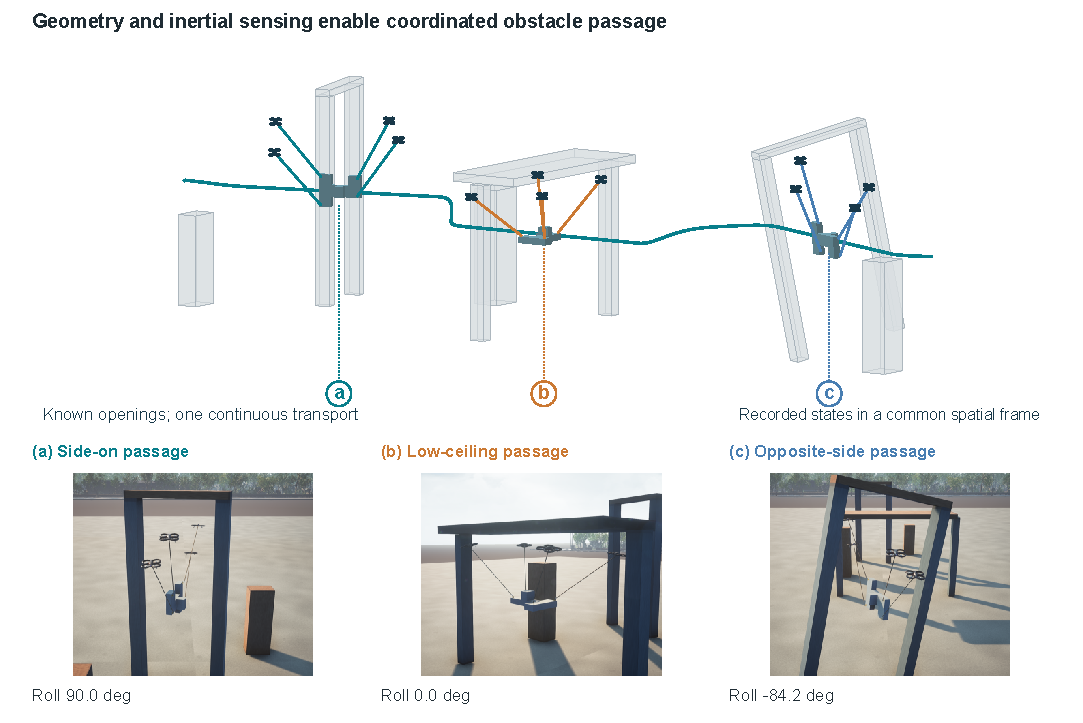
\includegraphics[width=\textwidth]{fig01_overview.pdf}
\caption{Cooperative transport through sequential spatial restrictions. The common-frame spatial view places three recorded payload and support configurations within the known obstacle course. Linked Unreal views show (a) side-on passage through the narrow opening, (b) a spread formation beneath the low ceiling, and (c) opposite-side passage through the tilted opening. Geometry and inertial observations supply the model used for force planning; the load attitude reference family is prescribed. The three configurations belong to one continuous closed-loop simulation.}
\label{fig:overview}
\end{figure*}

Geometry alone cannot determine whether a desired configuration can be sustained. The load center of mass (CoM) generally differs from the centroid of its visible surface, especially when equipment or dense material is distributed unevenly inside the object. A misplaced CoM changes the moment produced by every cable and therefore changes the tension distribution required for a given attitude. Rotational inertia further affects the moments needed during attitude transitions. Because each cable force also determines an aircraft's direction and distance from its attachment, an inertial modeling error changes both tracking behavior and the formation's spatial envelope.

Several strands of research address these issues. Vision and inertial sensing have been used for cooperative cable transport~\cite{li2021}, and nonlinear model predictive control coordinates transportation and load manipulation~\cite{nmpc2023}. Arab et al.~\cite{ast2021} study planning and distributed control for a nonuniform slung load. Load-distribution-based planning~\cite{geng2022} connects the distribution of lifting effort to multilift trajectories. These studies establish that load distribution is a relevant planning variable rather than a consequence to be checked only after a centerline path has been selected.

Agile manipulation also requires the full supporting system to remain feasible. Sun et al.~\cite{sun2025} demonstrate rapid cooperative manipulation using trajectory optimization and incremental nonlinear dynamic inversion. Their evaluations include substantial model mismatch and changing load properties. Thus, agile payload rotation and mismatch-tolerant tracking are established capabilities. Control barrier functions have been used in cooperative manipulation trajectory planning~\cite{pallar2025}, while PolyFly~\cite{polyfly2026} uses polytopic descriptions for collision-free suspended transportation. These approaches motivate evaluating the geometry of aircraft and cables together with that of the payload. Learning-based direct motor control provides another route to cooperative transport~\cite{crazymarl2026}; the present study uses an explicit mechanical model so that estimated moments can be traced through force allocation to formation geometry.

Recent AST studies further clarify the planning context. Chai et al.~\cite{chai2026} investigate time-optimal gap traversal for collaborative aerial transportation with experimental evaluation. Sun et al.~\cite{sunlocal2026} address local obstacle avoidance and trajectory tracking for multi-quadrotor transport. Chan et al.~\cite{chan2026} formulate time-optimal planning of a cable-suspended payload quadcopter using spatial reformulation. The present objective is complementary: given an aperture-conditioned rigid-payload reference family, infer inertial moments from virtual geometry, tension and motion measurements, then propagate them through a compliant force-to-endpoint model. Timing is selected from a finite set; global time optimality and autonomous discovery of the attitude sequence are outside this formulation.

Inertial estimation supplies the complementary information. Petitti et al.~\cite{petitti2020} combine suspended-load inertial estimation with energy-efficient cooperative control. Physically consistent identification relates rigid-body inertial parameters to moments of a nonnegative mass distribution~\cite{wensing2018}. Heins and Schoellig~\cite{heins2025} exploit uncertain inertial parameters and shape information in nonprehensile transportation. These results provide the basis for distinguishing external shape from internal mass properties. A surface scan supports spatial reasoning and constrains possible mass locations; force and motion observations are needed to identify the moments relevant to dynamics.

This paper addresses the connection between measured inertial information and feasible reconfiguration during obstacle passage. We consider a rigid object with calibrated cable attachment points, scanned before transport, and apertures whose geometry is known. The payload translation and attitude are parameterized by smooth, aperture-conditioned references. The planner determines the cable-force history and the resulting compliant endpoint trajectories, together with lowering and timing candidates. The aircraft then track these endpoints through motor and rigid-body dynamics using delayed visual pose feedback. This formulation makes the influence of an identified CoM explicit: it alters the required wrench distribution and, through cable directions, the formation needed to realize the maneuver.

The contribution is an explicit connection from identified inertial moments to constrained support geometry, evaluated under a prescribed payload reference family. First, a sensing-to-configuration formulation combines markerless surface registration, synchronized tension observations and shape-supported integral inertial identification. It provides the mass moments used by the same force and geometry model during transportation. Second, a smooth conic force planner accounts for compliant cable endpoints, aperture halfspaces and aircraft actuation. For near-vertical load attitudes, sequential endpoint separation preserves distinct aircraft positions while the attachment geometry changes orientation. Third, controlled simulations examine three-aircraft and four-aircraft teams, compare identified and uniform-shape models, and demonstrate successive large-angle reorientations of a nonconvex payload through a multi-aperture course. Numerical refinement and an independent continuous command replay examine the underlying mechanical computation.

\begin{figure*}[t]
\centering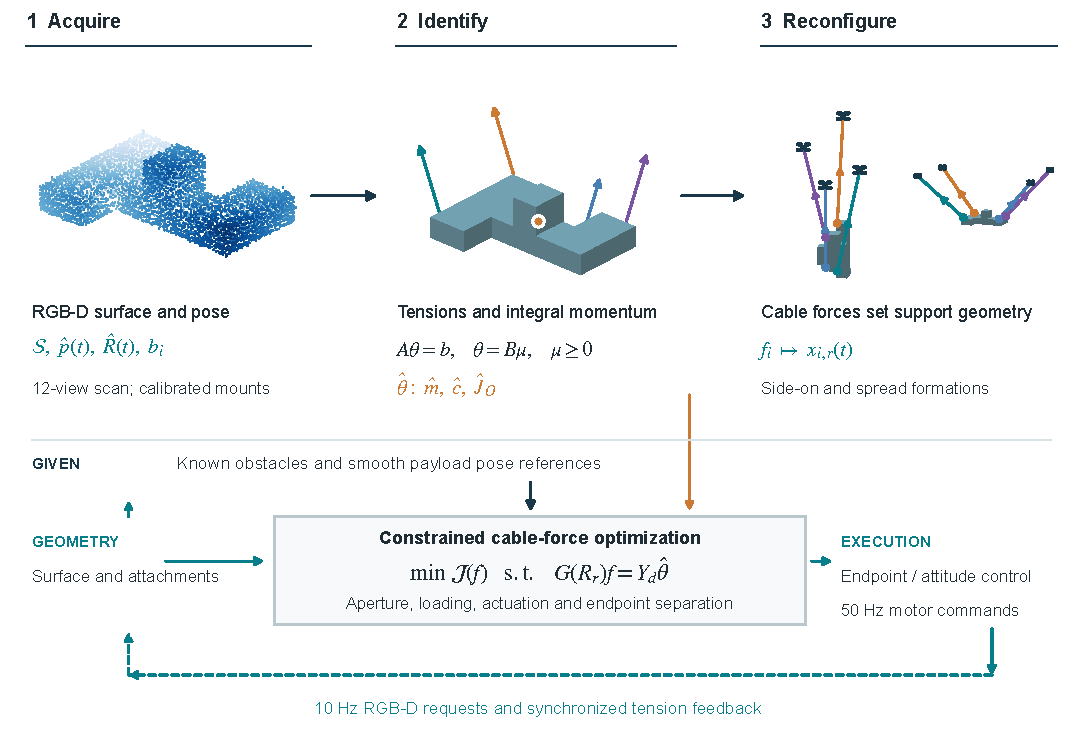
\includegraphics[width=\textwidth]{fig02_framework.pdf}
\caption{Information flow from acquired geometry to supporting formation. Surface and pose registration supplies a common geometric frame; integral momentum and tension observations supply the inertial moments. The known openings and prescribed smooth payload references enter constrained force optimization together with the reconstructed geometry and identified moments. The compliant endpoint map converts cable forces to supporting aircraft positions, followed by motor-driven feedback execution. Point clouds and support configurations use the forked-payload records. The return path denotes visual and tension feedback, rather than online attitude-sequence search.}
\label{fig:framework}
\end{figure*}

\section{Transport model and problem formulation}
\subsection{Payload geometry and attachment coordinates}
Consider $N\in\{3,4\}$ quadrotors carrying a rigid payload through $N$ individually attached cables. Let $p\in\R^3$ and $R\in\SO$ denote the position and orientation of a reference frame fixed to the scanned object. This frame is determined geometrically and need not coincide with the CoM. Let $b_i$ be the calibrated attachment coordinate in this frame, $x_i$ the aircraft cable endpoint, and $\mathcal{S}$ the reconstructed payload surface. The world attachment is
\begin{equation}
 a_i=p+Rb_i,\qquad d_i=x_i-a_i,\qquad q_i=\frac{d_i}{\norm{d_i}}.
 \label{eq:attachments}
\end{equation}
With tension $T_i\geq0$, the cable force acting on the payload is $f_i=T_iq_i$. Noncollinear attachment geometry is required. Installed attachment coordinates are supplied by rigging calibration; they are not inferred from the object's geometric centroid.

The environment is represented by oriented obstacle boxes $\mathcal{O}_j$. Collision evaluation considers the transformed surface $p+R\mathcal{S}$, each aircraft envelope and each complete cable segment $[a_i,x_i]$. The forked payload retains its open bays and protrusions in the collision model. A convex envelope is used separately for inertial support, as described in Section~\ref{sec:identification}.

\subsection{Rigid-body inertial parameters}
Let $m$ be the payload mass, $c$ its body-frame CoM coordinate and $J_O$ its inertia about the scan origin. The ten linear inertial parameters are
\begin{equation}
 \theta=\begin{bmatrix}m&h^T&j^T\end{bmatrix}^{T},\quad h=mc,
 \label{eq:theta}
\end{equation}
where $j$ contains the six independent entries of the symmetric matrix $J_O$. The inertia about the CoM is
\begin{equation}
 J_C=J_O-m\big(\norm{c}^{2}I-cc^T\big).
 \label{eq:parallel}
\end{equation}
Let $v=\dot p$, $\omega$ and $\alpha=\dot\omega$ be world-frame linear velocity, angular velocity and angular acceleration, and let $g=[0,0,-9.81]^T$ m/s$^2$. The cable wrench required about the scan origin satisfies
\begin{align}
 F&=m(\ddot p-g)+(\sk{\alpha}+\sk{\omega}^{2})Rh,\label{eq:force}\\
 \tau_O&=\sk{Rh}(\ddot p-g)+RJ_OR^T\alpha
                 +\omega\times(RJ_OR^T\omega).\label{eq:moment}
\end{align}
Consequently $w=[F^T,\tau_O^T]^T=Y_d(R,\omega,\ddot p,\alpha)\theta$ is linear in $\theta$. For stacked cable forces $f=[f_1^T,\ldots,f_N^T]^T$, the same wrench is
\begin{equation}
 G(R)f=w,\quad
 G(R)=\begin{bmatrix} I&\cdots&I\\\sk{Rb_1}&\cdots&\sk{Rb_N}\end{bmatrix}.
 \label{eq:wrenchmap}
\end{equation}
The translation--rotation coupling in Eqs.~\eqref{eq:force}--\eqref{eq:moment} is retained during both identification and planning. In particular, a CoM offset produces a moment even during low-acceleration translation.

\subsection{Compliant cables and aircraft dynamics}
The cables are modeled as unilateral spring--damper elements with rest length $\ell_0$, stiffness $k_c$ and axial damping $d_c$. With $\delta_i=\norm{d_i}-\ell_0$,
\begin{equation}
 T_i=\begin{cases}
 \max(0,k_c\delta_i+d_c\dot\delta_i),&\delta_i>0,\\
 0,&\delta_i\leq0.
 \end{cases}
 \label{eq:cable}
\end{equation}
This law applies equal and opposite forces to the load and aircraft. The aircraft translational dynamics take the form
\begin{equation}
 m_u\ddot p_i=u_i-f_i+m_ug-d_v\dot p_i,
 \label{eq:uav}
\end{equation}
where $u_i$ is the rotor-generated thrust vector. Each aircraft has a free rotational state, and motor-site forces generate the corresponding body moments. A first-order motor response filters each thrust command before it acts on the body. The physical integration therefore includes cable stretch, aircraft attitude response and motor lag.

\subsection{Planning objective}
Let $p_r(t;\eta)$ and $R_r(t;\eta)$ define an aperture-conditioned reference family, where $\eta$ selects the lowering and duration candidate. The problem is to find a smooth force sequence satisfying Eq.~\eqref{eq:wrenchmap}, cable loading limits and aperture conditions, and to convert that sequence into realizable aircraft endpoints. The complete endpoint and payload trajectories must satisfy the selected geometry and actuation checks. This finite candidate formulation specifies the motion family explicitly; obstacle geometry, attachment calibration and the acquired surface are inputs to the planner.

The coupling can be seen from the quasi-static endpoint map
\begin{equation}
 x_i=a_i+\left(\ell_0+\frac{\norm{f_i}}{k_c}\right)\frac{f_i}{\norm{f_i}}.
 \label{eq:endpointmap}
\end{equation}
Changing $\hat\theta$ changes the wrench in Eq.~\eqref{eq:wrenchmap}, the admissible $f_i$, and the endpoint $x_i$. Thus internal mass information influences the spatial formation even for an unchanged external shape and payload reference.

\section{Vision and tension based inertial identification}
\label{sec:identification}
\subsection{Surface reconstruction and visual pose}
The initial object scan is acquired in a known static installation fixture. Depth measurements are projected into calibrated coordinates and fused from twelve views. Voxel reduction produces a surface point set with up to 6000 points. The known fixture fixes the initial scan frame, including the orientation of a geometrically symmetric cuboid. Subsequent registration operates on the acquired surface rather than on a supplied ideal object mesh.

During transport, two virtual RGB-D views provide partial surface observations. A predicted search region follows the most recent registered pose, and geometric correspondence rejects points inconsistent with the reference surface. Point-cloud alignment follows the iterative registration principle~\cite{icp1992}; temporal prediction initializes each local alignment. For the forked object, chromaticity statistics learned during the fixture scan filter background points while preserving thin prongs and cavity boundaries. The initial scan precedes rope installation, while transport images include the rigging. No fiducial marker or renderer object-ID mask is used.

The resulting visual observations are timestamped by exposure time. Tensions and aircraft endpoint telemetry are sampled at the same time. Their association is retained when image processing finishes later. The estimator therefore uses cable directions and load pose from a common physical instant rather than combining delayed geometry with current tensions. Nine consecutive observations are fitted by a local cubic polynomial, with derivatives assigned to the center observation. At the 10 Hz request rate this introduces an approximately 0.4 s fixed lag. Only observations already received enter an identification solve. This 0.4 s derivative lag applies to preparation-phase parameter estimation. During transport, the controller uses the most recent visual pose and a velocity-based prediction to the current control time; its reported sensor age is the exposure-to-control age, without the preparation derivative lag.

\subsection{Integral momentum observations}
An integral formulation avoids differentiating the visual trajectory twice. About a fixed world origin, payload linear and angular momenta are
\begin{align}
 P&=mv+\omega\times Rh,\\
 H&=p\times P+(Rh)\times v+RJ_OR^T\omega.
 \label{eq:momentum}
\end{align}
Both are linear in $\theta$, so define $[P^T,H^T]^T=Y_M\theta$. Gravity contributes the parameter-linear wrench
\begin{equation}
 w_g=\begin{bmatrix}mg\\(mp+Rh)\times g\end{bmatrix}=Y_g\theta.
\end{equation}
The measured cable wrench about the same origin is
\begin{equation}
 w_c=\begin{bmatrix}\sum_i T_iq_i\\\sum_i a_i\times(T_iq_i)\end{bmatrix}.
\end{equation}
For every complete interval $[t_a,t_b]$, integration gives
\begin{equation}
 \left(Y_M(t_b)-Y_M(t_a)-\int_{t_a}^{t_b}Y_g\,dt\right)\theta
       =\int_{t_a}^{t_b}w_c\,dt.
 \label{eq:integral}
\end{equation}
The implementation uses trapezoidal integration over nonoverlapping 0.4 s intervals. Stacking the resulting equations produces $A\theta=b$. A translated fixed world origin near the first observation reduces unnecessary moment lever arms while preserving Eq.~\eqref{eq:integral}.

\subsection{Shape-supported moment fitting}
Let $s_r$ be candidate mass-support locations inside the convex hull of the reconstructed surface. A nonnegative mass $\mu_r$ at each location contributes to mass, first moments and inertia. With a small isotropic cell-inertia term $\epsilon I$, the contributions are
\begin{equation}
 m=\sum_r\mu_r,\quad h=\sum_r\mu_rs_r,\quad
 J_O=\sum_r\mu_r\big(\norm{s_r}^{2}I-s_rs_r^T+\epsilon I\big).
 \label{eq:support}
\end{equation}
Write these relations compactly as $\theta=B\mu$. The estimate is obtained from
\begin{equation}
 \begin{split}
 \min_{\mu}\;&\tfrac12\norm{AB\mu-b}^{2}+\tfrac{\lambda}{2}\norm{\mu}^{2}\\
 \text{s.t. }&\mu\geq0,\qquad m_{\min}\leq\mathbf{1}^{T}\mu\leq m_{\max}.
 \end{split}
 \label{eq:fit}
\end{equation}
This is a convex quadratic conic program~\cite{boyd2004}. The nominal fit minimizes the unwhitened residual in SI units. Linear- and angular-impulse residuals are reported separately. To assess the relative scaling of their different units, the supplementary analysis rescales moment rows by $1/L$ for $L\in\{0.25,0.5,1,2\}$ m and refits the same observations; this is a unit-weighting sensitivity test, not covariance whitening. The support spacing is 0.08 m, $\epsilon=5\times10^{-5}$ m$^2$, $\lambda=10^{-8}$, and the prescribed mass interval is 0.7--1.5 kg. A limited set of hull vertices supplements the interior grid. Nonnegative support guarantees moments realizable by mass within the scanned convex envelope, following the mass-distribution interpretation of inertial parameters~\cite{wensing2018}.

For a nonconvex object, this hull is a conservative envelope of possible mass locations. It serves the moment estimation problem, whereas the reconstructed nonconvex surface serves collision evaluation. The envelope therefore imposes moment consistency and a spatial outer bound, rather than identifying a material-only density. The weights in Eq.~\eqref{eq:fit} are one representation of the fitted moments: many different internal distributions can generate the same ten parameters. The estimated quantities passed to the planner are $\hat m$, $\hat c$ and $\hat J_O$.

An activation test checks the measurement geometry before using these moments. The normalized observation matrix must have rank ten, condition number at most 1000 and at least eight complete integral windows. The minimum eigenvalue of the mean $\omega\omega^T$ matrix must exceed $10^{-4}$ s$^{-2}$. Measured tension must exceed its 0.01 N error bound, and the central second-moment matrix $\frac12\operatorname{tr}(J_C)I-J_C$ must be positive definite. These conditions connect activation to angular excitation, valid tension measurements and physical moment consistency.

\begin{figure*}[t]
\centering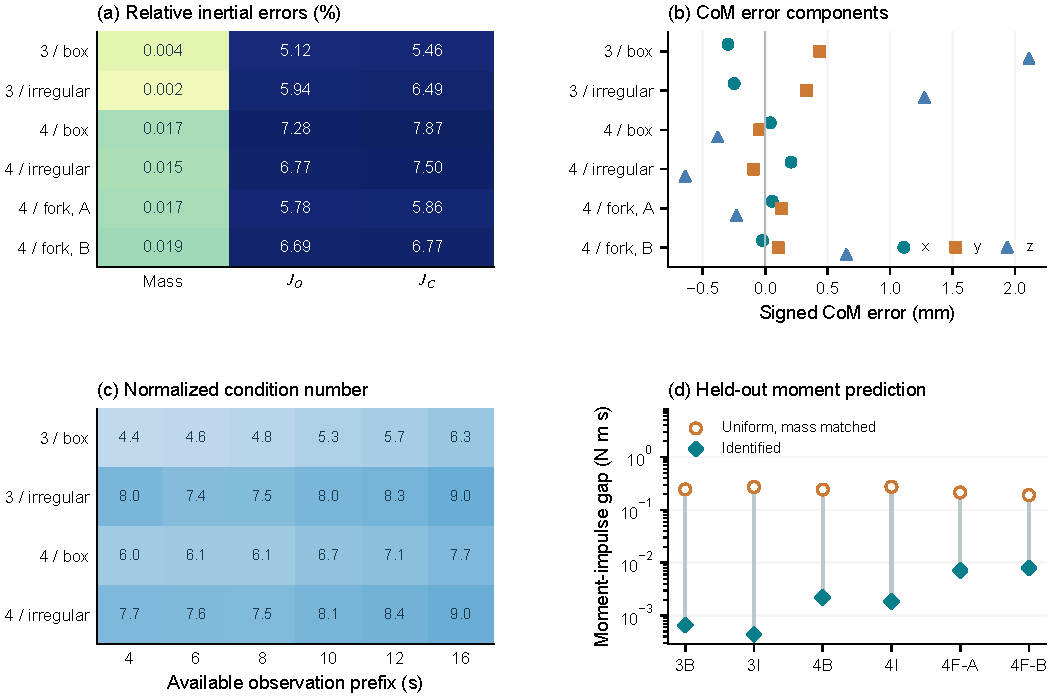
\includegraphics[width=\textwidth]{fig03_identification.pdf}
\caption{Inertial accuracy and predictive evaluation. (a) Relative mass and inertia errors in six recorded executions; inertia errors use the Frobenius norm. (b) Signed CoM errors in the scan frame; circles, squares and triangles denote the $x$, $y$ and $z$ components. (c) Condition number of the column-normalized integral observation matrix using only data available by each prefix; all displayed systems have rank ten. (d) RMS difference from the true-inertia moment-impulse prediction on transport observations excluded from fitting, comparing identified and mass-matched uniform models. Fork A and B denote the moderate- and large-rotation courses. Heatmap colors use logarithmic scales; cell annotations give the numerical values.}
\label{fig:identification}
\end{figure*}

\section{Coupled force and formation planning}
\subsection{Aperture-conditioned motion references}
The inputs are the reconstructed surface, calibrated attachments, known obstacle boxes, fitted inertial parameters and a prescribed smooth payload reference family. The continuous optimization variables are the three components of every cable force at each time node. Duration and lowering are selected by ordered finite candidate search. Payload position and attitude follow the selected reference; aircraft endpoints are derived from optimized forces and cable stretch. Thus force allocation and support formation adapt to the measured load, while the obstacle-crossing attitude sequence is supplied by the reference family.

The load reference is represented by smooth translation and attitude functions over a selected duration $D$. The basic experiment translates the payload by 8 m while moving toward a terminal roll, pitch and yaw of $25^\circ$, $10^\circ$ and $30^\circ$. The reference includes a smooth lowering window under the beam. Candidate durations are 20, 22, 25 and 30 s; candidate lowering values are evaluated in a fixed order.

For sequential apertures, a piecewise quintic centerline connects their approach and exit neighborhoods. Smooth activation functions blend the associated attitude references. In the large-angle course the sequence is horizontal, $90^\circ$ roll at the narrow aperture, horizontal with $90^\circ$ yaw under the ceiling, $-85^\circ$ roll at the tilted aperture, and return to the nominal attitude. The references vary during forward motion. Their activation regions extend across the occupied aperture neighborhood, so a load transition is not released while supporting aircraft still occupy the frame. Duration and lowering candidates are evaluated using the same force and endpoint checks.

\subsection{Smooth conic cable-force optimization}
At time nodes $t_j$, let $f_j\in\R^{3N}$ contain the load cable forces, and let $f_j^0$ be a preferred outward preload. For a chosen motion candidate, the force planner minimizes
\begin{equation}
 \begin{split}
 \mathcal{J}(f)=&\frac{0.02}{2}\norm{f-f^0}^{2}
 +\frac{0.04}{2}\norm{D_1f}^{2}\\
 &+\frac{0.20}{2}\norm{D_2f}^{2}
 +\frac{0.04}{2}\norm{D_3f}^{2},
 \end{split}
 \label{eq:objective}
\end{equation}
where $D_1,D_2,D_3$ are time-scaled first, second and third finite-difference operators. Force equilibrium is imposed at every node:
\begin{equation}
 G(R_r(t_j))f_j=Y_d(t_j)\hat\theta.
 \label{eq:equilibrium}
\end{equation}
The formulation includes upward force, tension and nominal thrust cones,
\begin{equation}
 f_{ij,z}\geq0.55,\quad \norm{f_{ij}}\leq8.2,\quad
 \norm{f_{ij}+m_ug_0 e_z}\leq29.5,
 \label{eq:cones}
\end{equation}
with forces in newtons, $e_z=[0,0,1]^T$, and $g_0=9.81$ m/s$^2$ denoting the positive gravity magnitude. In the thrust cone, $m_ug_0e_z=-m_u g$ with the vector convention of Section 2. The 29.5 N cone limits nominal total thrust; four 7.5 N motor limits permit 30 N total before moment allocation. Dynamic endpoint verification applies a tighter 28 N nominal limit. Componentwise limits of 8 N/s and 25 N/s$^2$ are placed on the first and second differences. Near-zero first differences at the endpoints reduce force transients when joining the preparation and transport phases. The initial force is projected onto the first wrench equality to maintain continuity.

An outward preload prevents the formation from collapsing above the object. For large roll angles, horizontal aircraft sectors are defined using a horizontal projection of the payload longitudinal axis and its orthogonal horizontal direction. The sectors retain the original attachment ordering when the attachment plane becomes nearly vertical. Side-force conditions are relaxed with increasing roll to allow the force couples required by the upper and lower attachments. The subsequent endpoint and cable checks determine acceptance.

\subsection{Aperture constraints and compliant endpoints}
For an aperture halfspace $n^Tx_i\leq\beta$ and known attachment $a_i$, define the endpoint allowance $c_i=\beta-n^Ta_i>0$. A conservative linear force condition used in the conic problem is
\begin{equation}
 \left(n-\frac{c_i}{\ell_{\max}}v_i\right)^Tf_i\leq0,
 \label{eq:halfspace}
\end{equation}
where $v_i$ is a prescribed unit direction and $\ell_{\max}=2.05$ m bounds the planned cable length. Since $v_i^Tf_i\leq\norm{f_i}$, this condition implies $n^Tf_i\leq(c_i/\ell_{\max})\norm{f_i}$. Together with $\ell_i\leq\ell_{\max}$, it bounds the nonlinear endpoint displacement toward the halfspace. Height limits are expressed by related outward/upward force inequalities. Full nonlinear geometry is checked after solving.

For a smooth force magnitude $T_i(t)=\norm{f_i(t)}$, stretch is computed from
\begin{equation}
 d_c\dot\delta_i+k_c\delta_i=T_i(t),\qquad
 x_{i,r}=p_r+R_rb_i+(\ell_0+\delta_i)\frac{f_i}{T_i}.
 \label{eq:stretch}
\end{equation}
The stretch dynamics are propagated at 5 ms resolution, and clamped cubic splines supply the endpoint position, velocity and acceleration. This step retains axial damping instead of instantaneously changing cable length whenever tension changes. Aircraft acceleration, dynamic thrust and tilt are evaluated on the resulting endpoint curves, supplementing the nominal cones in Eq.~\eqref{eq:cones}.

\subsection{Separation during large-angle reorientation}
Near-vertical payload orientations can bring different endpoint directions close together even when the attachments themselves are well separated. We therefore add sequential linearized endpoint separation. At a preceding force solution $\bar f_i$, the static elastic map in Eq.~\eqref{eq:endpointmap} has Jacobian
\begin{equation}
 J_i=\frac{\ell_0}{\norm{\bar f_i}}\left(I-\bar q_i\bar q_i^T\right)+\frac{1}{k_c}I.
 \label{eq:jacobian}
\end{equation}
For the previous endpoint difference direction $n_{i\ell}$, impose
\begin{equation}
 n_{i\ell}^{T}\left[\bar x_i+J_i(f_i-\bar f_i)
 -\bar x_\ell-J_\ell(f_\ell-\bar f_\ell)\right]\geq d_{\rm lin}.
 \label{eq:separation}
\end{equation}
Three successive conic updates use $d_{\rm lin}=0.72$ m. The final damped endpoint trajectory is then evaluated nonlinearly. Its acceptance distance is 0.52 m; the linearization distance is an optimization reference rather than a guaranteed executed separation. This distinction matters because damping, spline interpolation and tracking alter the static linearization geometry.

Feasibility is evaluated at three distinct levels. The conic solve enforces nodal wrench equalities and force cones. Candidate verification evaluates damped, interpolated endpoints and complete geometric occupancy. Closed-loop execution is assessed using the measured tracking, loading and actuation limits in Section 5. The 0.72 m separation linearization reference encourages spacing during optimization; the nonlinear candidate gate is 0.52 m. Execution reports aircraft center distance separately from clearance after subtracting the collision envelope. Preparation transients are also included in execution tension extrema; they are not subject to the transport-only force reference bound.

The course uses 121 force nodes. Final evaluation samples the full acquired surface, aircraft envelopes and complete cable segments at 20 ms intervals, with actuation evaluation on the finer endpoint curve. A candidate is accepted only after its nonlinear force, geometry, speed and acceleration checks pass. Accepted course references satisfy aircraft speed below 2.5 m/s, reference acceleration below 2.75 m/s$^2$, tension between 1 and 8.25 N, dynamic thrust below 28 N and tilt below $37^\circ$. The single-beam reference acceleration budget is 2.25 m/s$^2$. These budgets leave room for tracking corrections in the execution loop.

\subsection{Closed-loop execution}
At each control instant, a delayed registered load pose is propagated using its available velocity estimate and combined with current aircraft telemetry. A low-pass payload pose correction shifts the endpoint references. Wider corner mounts use a lower visual pose gain to keep delayed rotational corrections below the coupled load-swing response. The aircraft command is
\begin{equation}
 u_i=m_u\left(\ddot x_{i,r}+K_p(x_{i,r}+\Delta_i-x_i)
      +K_v(\dot x_{i,r}-\dot x_i)-g\right)+f_i+d_v\dot x_i,
 \label{eq:controller}
\end{equation}
where $K_p=18I$ s$^{-2}$ and $K_v=7I$ s$^{-1}$, $\Delta_i$ is the filtered pose correction, and requested acceleration is capped at 4.5 m/s$^2$. A geometric attitude controller~\cite{lee2010} aligns each aircraft's thrust direction with this command, followed by allocation to four filtered motor inputs.

Image registration runs in its own worker. Identification and whole-segment planning run in a separate process; the aircraft remain under preparation/hover control while these computations finish. After the candidate is ready, the transport clock starts and the 50 Hz feedback loop follows its reference. This arrangement assigns explicit computation and observation times to the complete sensing--planning--execution chain.

\section{Simulation experiments}
\subsection{Experimental setup and evaluation criteria}
The dynamic simulator integrates the payload and every aircraft as free rigid bodies in MuJoCo~\cite{mujoco2012}. Individual rotor-site forces generate aircraft translation and rotation, and the cable law in Eq.~\eqref{eq:cable} generates the load reactions. Table~\ref{tab:parameters} summarizes the model and sensing settings. The default physical integration step is 0.5 ms, and motor commands are updated at 50 Hz. Computation is executed on a workstation with an AMD Ryzen 9 8945HX processor and an NVIDIA GeForce RTX 5070 Ti Laptop GPU.

\begin{table}[t]
\centering\small
\caption{Dynamic and sensing parameters. Noise bounds apply to the corresponding virtual measurements.}
\label{tab:parameters}
\begin{tabular}{@{}ll@{}}\toprule
Quantity & Value\\\midrule
Aircraft mass & 1.0 kg\\
Aircraft inertia diagonal & $[.009,.009,.016]$ kg m$^2$\\
Cable rest length & 2.0 m\\
Cable stiffness / damping & 180 N/m / 5 N s/m\\
Maximum thrust per motor & 7.5 N\\
Motor response time constant & 25 ms\\
Aircraft linear drag coefficient & 0.2 N s/m\\
Local ICP RMSE / inlier gate & 18 mm / 0.65\\
Correspondence gate & 80 mm\\
Control / RGB-D request rate & 50 Hz / 10 Hz\\
RGB-D image resolution & $256\times192$ pixels per view\\
Depth noise standard deviation & 1 mm\\
Tension noise & Uniform $\pm0.01$ N\\
Aircraft position noise & Uniform $\pm0.5$ mm\\
Preparation motion & 16 s\\
Physical integration step & 0.5 ms\\\bottomrule
\end{tabular}
\end{table}

Two complementary task groups are evaluated. The base group comprises rectangular and nonconvex stepped payloads, each carried by three and four aircraft, as illustrated in Fig.~\ref{fig:configurations}. Each configuration is paired with a uniform-shape control model, giving eight task attempts. Within each pair, the object, hidden ballast, sensor seed, preparation procedure and planning rules are held fixed. The uniform model distributes a nominal 1.05 kg over interior scan-support locations, while the identification model uses Eq.~\eqref{eq:fit}. The comparison therefore evaluates the inertial information supplied to planning and feedback under the same acquired external geometry.

\begin{figure*}[t]
\centering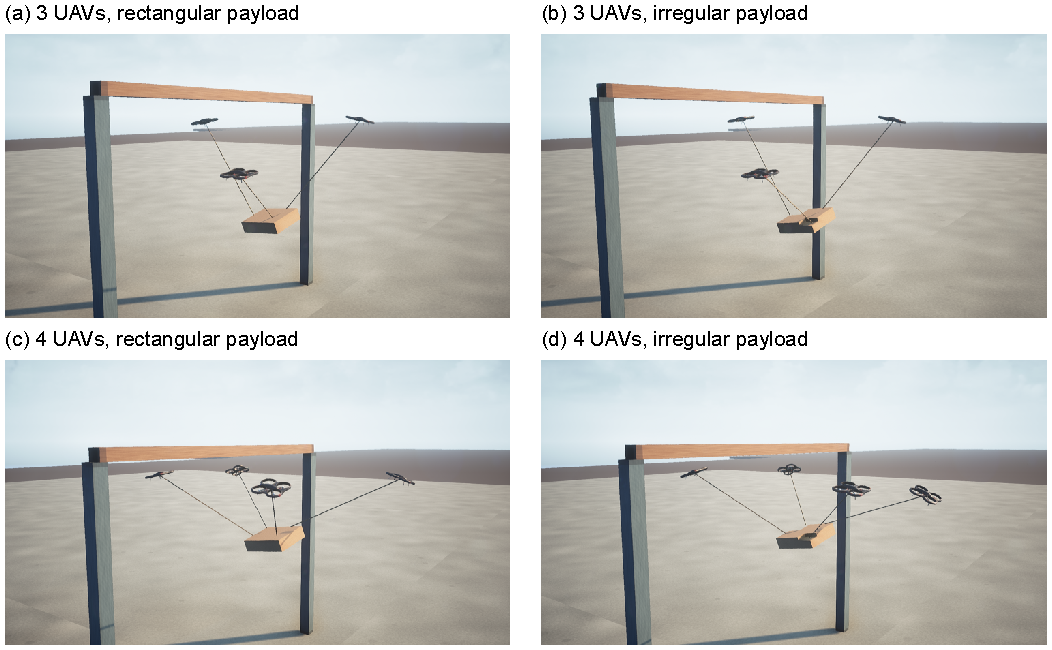
\includegraphics[width=.90\textwidth]{fig04_configurations.pdf}
\caption{Team-size and shape configurations in the base experiments. (a),(b) Three UAVs carrying rectangular and irregular payloads. (c),(d) The corresponding four-UAV configurations. All panels use original Unreal images of the recorded dynamic executions.}
\label{fig:configurations}
\end{figure*}

The second group carries a forked payload through sequential restrictions. The object measures $1.21\times0.90\times0.40$ m and has unequal side arms, open bays and a raised boss. Four mounts are installed at material-supported outer corners. Fixed padeyes, rotating shackles and rope terminations share the same attachment geometry as the force model. Mount mass and inertia are included in the load properties. The effective 2 m cable includes the 60 mm rigid termination, with the force application point at its pin center. These details permit large rotations while maintaining consistent visual and mechanical attachments.

Execution acceptance requires completed transport, peak position error at most 0.10 m, peak rotation error at most $5^\circ$, and tensions strictly between 0.5 and 9 N. Additional limits are $40^\circ$ aircraft tilt, 7.5 N per motor, 2.6 m/s aircraft speed and 6 m/s$^2$ aircraft acceleration. Rotation error is the magnitude of the logarithm of $RR_r^T$. Rigid-body contacts are monitored at physical substeps. Complete cable-segment checks use the 50 Hz records; the course clearance analysis inflates segment radius by the termination width and half a sampling interval of endpoint motion. Corresponding obstacle and load-body checks use the complete saved segment, rather than only cable endpoints.

The RGB-D inputs used for identification and feedback are rendered from the dynamic state and returned through the image-processing interface. Separately, Unreal Engine 5.2 and the CityPark Showcase environment produce the presentation images and videos. The distinction follows the useful separation between visual and physical simulation~\cite{airsim2017}: in this study numerical performance is measured from the MuJoCo closed loop, and Unreal displays those recorded states. The video output is $1920\times1080$ at 25 frames/s with one-to-one physical time. No display interpolation changes the recorded motion.

\subsection{Complete inertial identification and held-out prediction}
Across the four base configurations and two forked-payload executions, mass relative error is 0.0024--0.0188\%, and the CoM-inertia Frobenius relative error is 5.46--7.87\%. True and estimated mass, three-axis CoM, all six origin-inertia entries and principal moments are provided in the public numerical records. Figure~\ref{fig:identification}(a),(b) therefore evaluates the complete ten-parameter model rather than using CoM accuracy as a proxy for inertia accuracy. 
Figure~\ref{fig:identification} compares the models used for transportation. The identified CoM errors range from 0.39 to 2.18 mm across the four configurations. In contrast, the uniform-shape models differ from the actual CoM by approximately 103--117 mm. The external shape and installation coordinates are available to both models, so this difference concerns internal mass moments rather than surface acquisition.

Figure~\ref{fig:identification}(c) evaluates observation geometry at causal prefixes from 4 to 16 s. The normalized systems have rank ten, with condition numbers of approximately 4.4--9.0. At a 6 s prefix, the original activation criteria are satisfied in all four base cases. The prefix calculations share the original observation streams and quantify information availability during preparation.

For predictive evaluation, complete 0.4 s integral windows are formed from transport-only observations, excluding the first and last second of transport. These samples do not enter the preparation fit. Figure~\ref{fig:identification}(d) compares each model's predicted moment impulse against the true-inertia prediction on the same held-out regressor. Matching the uniform model's total mass isolates its remaining first- and second-moment errors. The repository also reports measured impulse residuals for both the fitted and true-inertia models, so parameter-model discrepancy can be distinguished from observation and integration residuals.

The completed four-aircraft rectangular pair provides a direct tracking comparison. Its uniform model has 102.75 mm CoM error and $22.05^\circ$ peak attitude error. With the identified model, these values are 0.39 mm and $0.66^\circ$. Peak translation error decreases from 8.19 to 2.76 cm. Thus the attitude error is reduced by approximately 97\% for this pair. The change has a mechanical explanation: a misplaced CoM creates an incorrect gravity moment in Eq.~\eqref{eq:moment}, which produces inappropriate cable-force distribution during rotation and load lowering.

\begin{figure*}[t]
\centering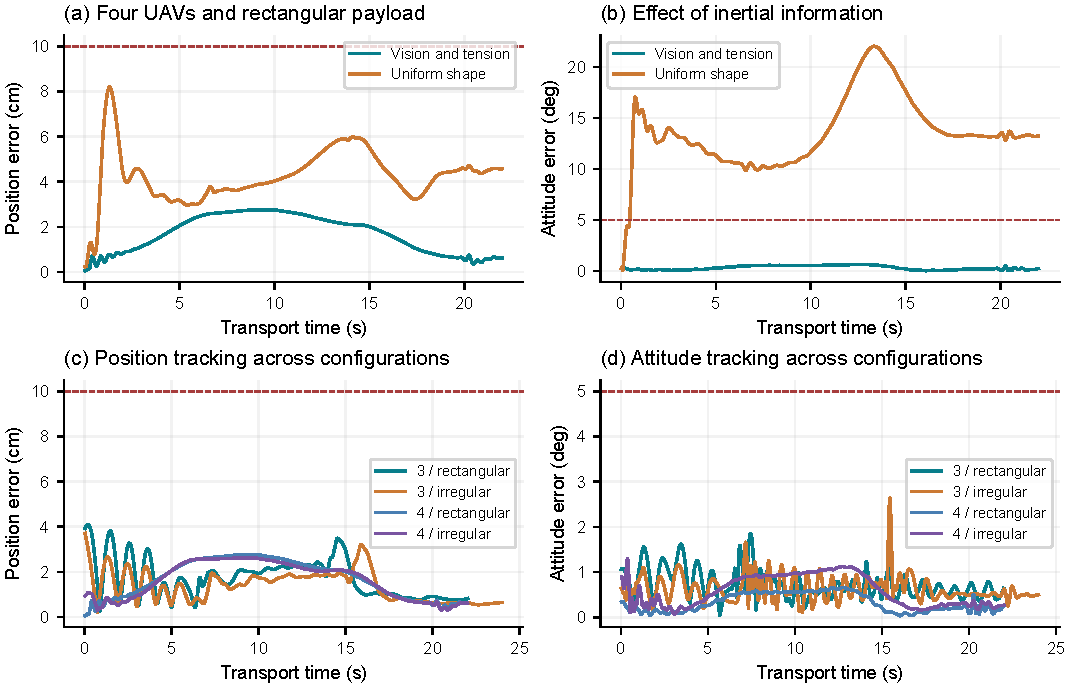
\includegraphics[width=\textwidth]{fig05_tracking.pdf}
\caption{Closed-loop tracking in the base experiments. (a),(b) Paired four-aircraft rectangular-payload executions with uniform-shape and identified inertial models. (c),(d) Identified-model position and rotation errors for all four team/shape configurations. Dashed lines mark the execution thresholds. Time is relative to each transport start.}
\label{fig:tracking}
\end{figure*}

\begin{table*}[t]
\centering\small
\caption{Base transport results with identified inertial moments. Each row is one executed team/shape configuration. Tension extrema include the complete preparation and transport at physical substeps.}
\label{tab:matrix}
\begin{tabular}{@{}clrrrrl@{}}\toprule
UAVs & Payload & Transport (s) & CoM error (mm) & Peak position (cm) & Peak attitude ($^\circ$) & Tension (N)\\\midrule
3 & Rectangular & 20 & 2.18 & 4.10 & 1.85 & 1.08--8.38 \\
3 & Irregular & 22 & 1.34 & 3.71 & 2.64 & 1.20--7.55 \\
4 & Rectangular & 20 & 0.39 & 2.76 & 0.66 & 1.63--8.69 \\
4 & Irregular & 20 & 0.68 & 2.62 & 1.29 & 1.03--8.61 
\\
\bottomrule\end{tabular}
\end{table*}

\subsection{Team size and payload geometry}
All four identified-model configurations satisfy the execution criteria. Table~\ref{tab:matrix} reports their individual results rather than treating them as repeated samples of one configuration. Peak position errors are 2.62--4.10 cm, and peak attitude errors are $0.66$--$2.64^\circ$. The three-aircraft irregular case selects 22 s from the candidate duration set; the other three use 20 s. Their peak payload speeds are 0.90--0.99 m/s, and average speeds within the central passage region are 0.84--0.93 m/s.

Figure~\ref{fig:tensions} shows cable loading during transportation. Across preparation and transport, tensions remain between 1.03 and 8.69 N. Aircraft, payload and cable-obstacle contacts are absent, and none of the identified-model runs saturates its motor commands. The four-aircraft rectangular formation reduces the vertical endpoint-to-payload envelope from a maximum of 1.94 m to a minimum of 1.09 m during the maneuver, while the endpoint lateral span varies between 1.86 and 3.38 m. The formation therefore changes the occupied vertical space by spreading the support directions as the payload passes beneath the beam.

\begin{figure*}[t]
\centering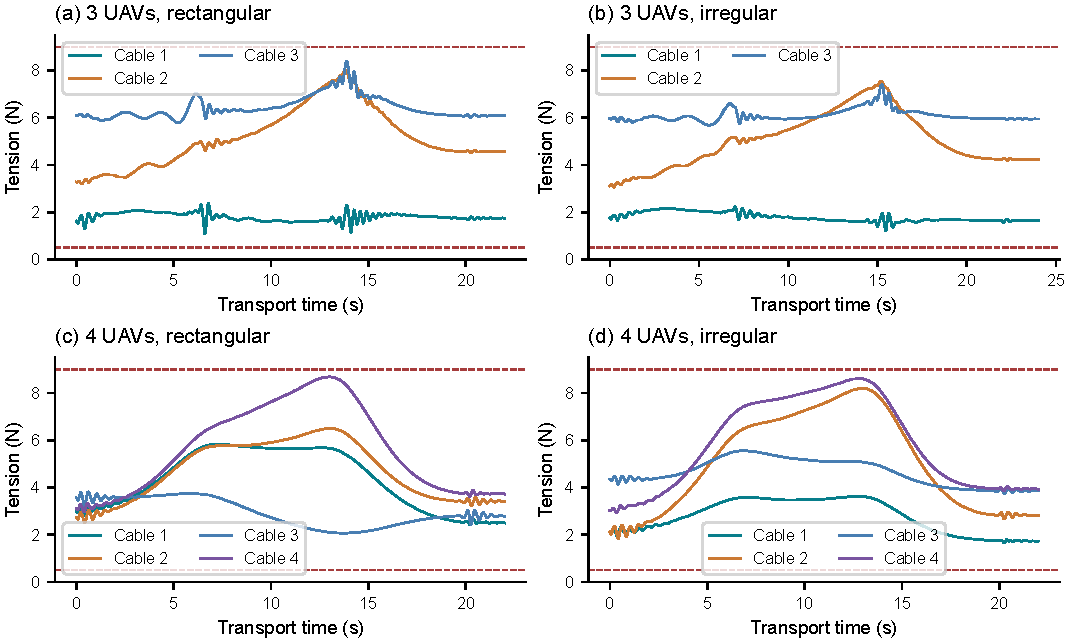
\includegraphics[width=\textwidth]{fig06_tensions.pdf}
\caption{Cable tensions during transport for the four identified-model configurations. Curves show 50 Hz saved states; dashed bounds are the 0.5--9 N execution limits. The extrema in Table~\ref{tab:matrix} additionally cover every physical substep and the preparation phase.}
\label{fig:tensions}
\end{figure*}

\begin{table*}[t]
\centering\small
\caption{Paired uniform-shape and identified-model outcomes under the same task rules. ``Planning rejection'' denotes that the candidate set did not produce an accepted force/geometry/actuation trajectory for that model.}
\label{tab:baseline}
\begin{tabular}{@{}clrlc@{}}\toprule
UAVs & Payload & Uniform CoM error (mm) & Uniform-model outcome & Identified outcome\\\midrule
3 & Rectangular & 103.35 & Planning rejection & Accepted \\
3 & Irregular & 115.31 & Planning rejection & Accepted \\
4 & Rectangular & 102.75 & Attitude limit exceeded & Accepted \\
4 & Irregular & 116.74 & Planning rejection & Accepted 
\\
\bottomrule\end{tabular}
\end{table*}

The uniform-model outcomes in Table~\ref{tab:baseline} complement the tracking example. Three configurations do not obtain an accepted candidate. The completed four-aircraft rectangular execution exceeds the attitude and aircraft acceleration limits. This comparison shows that the scanned outline alone does not provide the same task model as the outline augmented by measured inertial moments. Candidate rejection here is a result of the specified finite search, not a claim of global infeasibility of the physical task.

\subsection{Controlled ablations and sensor-seed repetitions}
The controlled comparison uses five inertial-information levels on each of the four base configurations: a uniform-shape model with true total mass; identified mass with uniform-shape CoM and central inertia; identified mass and CoM with mass-scaled uniform-shape central inertia; full identification; and true inertial parameters. All arms use the same acquired-geometry procedure, fixed ballast, sensor seed, preparation, reference family, candidate budget and feedback gains. The true-mass arm isolates errors in the first and second moments without a mass mismatch. The oracle is an information reference, rather than a competing planner.

\begin{table*}[t]
\centering\small
\caption{Five-arm controlled ablation. Entries give peak attitude error ($^\circ$) for completed executions. R denotes candidate planning rejection; A denotes an image-age abort before transport. Asterisks mark completed executions outside the common acceptance criteria. Each cell is one initial attempt, with all attempt records retained.}
\label{tab:ablation}
\begin{tabular}{@{}clrrrrr@{}}\toprule
UAVs & Payload & True mass, uniform & Mass only & Mass + CoM & Full identification & True inertia\\\midrule
3 & Rectangular & R & R & 1.75 & 1.81 & 1.80\\
3 & Irregular & R & R & A & 2.60 & 2.51\\
4 & Rectangular & 29.66\textsuperscript{*} & 29.44\textsuperscript{*} & 0.73 & 0.71 & 0.68\\
4 & Irregular & R & R & 1.16 & 1.06 & 1.14
\\
\bottomrule\end{tabular}
\end{table*}

Table~\ref{tab:ablation} distinguishes candidate availability from completed-transport accuracy. Both uniform-moment arms produce a candidate only for the four-aircraft rectangular configuration; its peak attitude errors are $29.66^\circ$ and $29.44^\circ$, respectively. All four full-identification and four true-inertia attempts satisfy the execution criteria. Three mass--CoM attempts complete and satisfy the criteria; the remaining acquisition abort is reported separately. In the four-aircraft rectangular case, their attitude peaks are $0.731^\circ$, $0.712^\circ$ and $0.678^\circ$. The dominant tracking gain in this task therefore follows CoM correction. The incremental effect of identifying central inertia is smaller and depends on the configuration; the three-aircraft rectangular mass--CoM arm, for example, has a slightly smaller attitude peak than its full-identification counterpart. Complete-inertia accuracy is assessed separately by Fig.~\ref{fig:identification} and transport-only prediction.

The three-aircraft irregular mass--CoM initial attempt stops on the image-age gate before transport and is retained as A, rather than classified as planning rejection. A separately labeled acquisition retry completes the task with a $2.54^\circ$ attitude peak. It does not replace the original table entry.

Twenty additional initial attempts use independent virtual sensor seeds for the fixed four-aircraft rectangular task. All 20 obtain an initial plan; 16 complete and satisfy the execution criteria, while 4 stop on the image-age gate. The all-attempt completion-and-acceptance rate is 16/20 (80\%; Wilson 95\% interval 58.4--91.9\%). Among the 16 complete transports, peak attitude error is $0.606$--$0.851^\circ$, and its median is $0.725^\circ$. Transport-only position RMS has median 1.96 cm and p95 1.97 cm; attitude RMS has median $0.427^\circ$ and p95 $0.488^\circ$. Initial planning time among complete transports has median 1.84 s and p95 1.89 s. These distributions are conditional on completed transport, and the initial attempts remain the statistical cohort even when a separately labeled diagnostic retry is available. The repeated task fixes shape and ballast; its seed distribution concerns sensing and acquisition timing under that configuration.

\subsection{Observation and support-model sensitivity}
Two archived preparation records, the four-aircraft rectangular case and the large-angle forked case, are each refitted under four declared measurement perturbations and twenty seeds per perturbation. The 160 fits isolate added pose noise (2 mm translation and $0.15^\circ$ rotation standard deviations), tension noise and bias (0.02 N each), fixed pose-frame bias (3 mm and $0.1^\circ$), and random observation removal (20\%). These synthetic ranges define a record-space sensitivity analysis; they do not represent hardware calibration or newly executed occluded-image flights. For the forked case, CoM-error p95 is 4.76 mm with added pose noise, 5.50 mm with tension perturbation, 2.25 mm with frame bias and 0.89 mm with observation removal. The corresponding central-inertia error p95 values are 19.52\%, 14.56\%, 11.05\% and 11.60\%. The full distributions for both records are available with the analysis protocol.

Changing $\lambda$ from $10^{-10}$ through $10^{-8}$ and $10^{-6}$ to $10^{-4}$ across all six nominal records changes CoM-error norms by at most 0.038 mm and central-inertia relative errors by at most 0.092 percentage points. A separate post-execution diagnostic restricts support locations to the evaluator's occupied body material for the two forked records. Central-inertia errors become 5.85\% and 6.72\%, compared with 5.86\% and 6.77\% for the acquired-surface hull. This comparison tests the moment envelope under the same observed motion; evaluator material geometry is used only in this diagnostic.

\subsection{Sequential apertures and large-angle reorientation}
The course comprises a 28 m centerline and twelve oriented solid obstacles: a laterally offset narrow frame, a low ceiling, a tilted frame, and three staggered blocks along the approach and exit regions. Figure~\ref{fig:course} shows the actual load and aircraft trajectories relative to these obstacles. Two course executions use the same forked object and corner mounts. The moderate-rotation course has a 2.70 m first opening and an 85 s transport. The large-rotation course narrows this opening to 2.10 m and uses a 125 s transport. The ceiling underside is 4.45 m above the ground, and the tilted opening has 2.85 m clear width.

\begin{figure*}[t]
\centering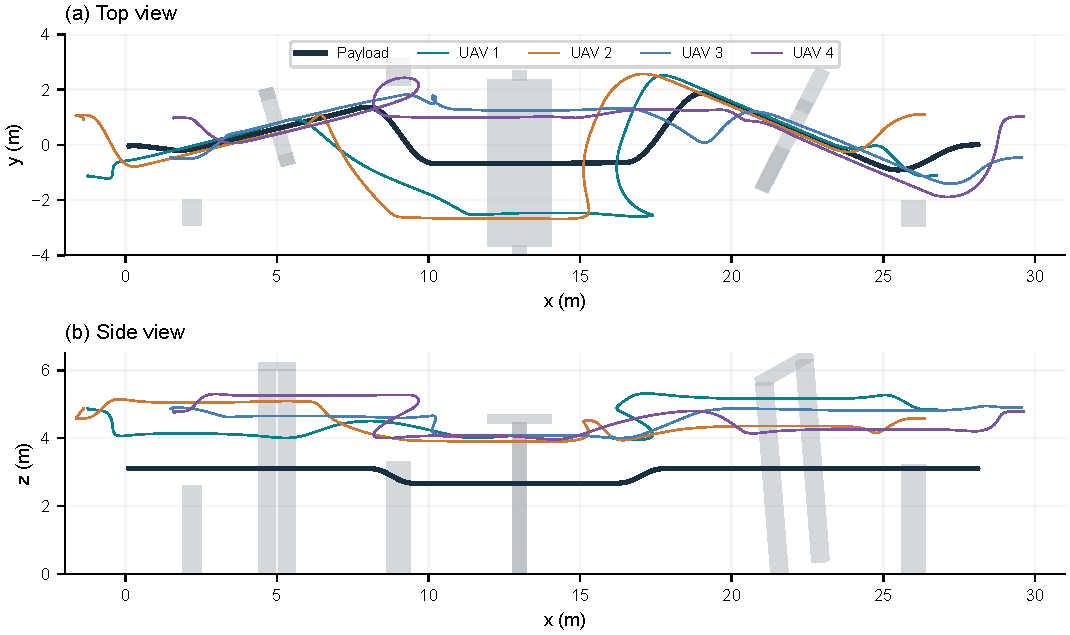
\includegraphics[width=\textwidth]{fig07_course.pdf}
\caption{Actual large-rotation course trajectories in (a) top and (b) side views. Gray polygons are projections of the twelve oriented obstacle boxes. The payload centerline and all four aircraft centers are plotted from the same dynamic execution.}
\label{fig:course}
\end{figure*}

In the large-rotation execution, the load is nearly horizontal at the start, rotates side-on for the first frame, returns to horizontal while changing heading under the ceiling, and rolls toward the opposite side for the last opening. Figure~\ref{fig:overview}(a)--(c) displays the three crossing configurations. The actual roll ranges from $-86.64^\circ$ to $90.34^\circ$, and yaw ranges from $-25.25^\circ$ to $90.85^\circ$. At the three crossing instants the roll angles are $90.03^\circ$, $0.03^\circ$ and $-84.24^\circ$. These rotations are achieved through cable loading while the team progresses along the course.

Figure~\ref{fig:course_dynamics} relates these attitudes to the supporting formation. The maximum vertical aircraft span is 1.37 m; it falls to approximately 0.19 m at the low-ceiling crossing. The minimum inter-aircraft separation over the complete execution is 0.640 m. The formation is consequently layered during side-on support and flattened under the ceiling. Payload attitude, relative aircraft position and available space change together.

\begin{table*}[t]
\centering\small
\caption{Forked-payload course executions. The two tasks have different first-aperture widths and prescribed rotation amplitudes; each is evaluated against the common execution criteria.}
\label{tab:course}
\begin{tabular}{@{}lrrrlrr@{}}\toprule
Course & Transport (s) & Peak position (cm) & Peak attitude ($^\circ$) & Tension (N) & Min. separation (m) & Planning (s)\\\midrule
Moderate rotation & 85 & 4.06 & 1.73 & 2.11--4.89 & 0.946 & 14.69 \\
Large rotation & 125 & 3.34 & 2.19 & 2.11--4.75 & 0.640 & 24.85 
\\
\bottomrule\end{tabular}
\end{table*}

Table~\ref{tab:course} reports the course results. The large-rotation execution has a 3.34 cm peak position error and $2.19^\circ$ peak attitude error. Tensions remain between 2.11 and 4.75 N, maximum aircraft tilt is $16.13^\circ$, and maximum aircraft speed is 2.38 m/s. The actual payload peak speed is 1.05 m/s. There are no rigid-body contacts, sampled cable-obstacle or cable-body intersections, slack cables or motor saturation intervals. All 1682 processed visual observations are valid under the registration tests.

The large-rotation geometric audit finds 0.081 m minimum aircraft clearance after a 0.28 m envelope inflation and 0.268 m minimum scanned-surface clearance after 0.045 m inflation. Complete cable segments are checked with a 0.0468 m radius including termination width and observed half-sample motion. These are sampled geometric margins with the stated motion inflation; they are not a general continuous-time safety certificate under arbitrary execution disturbances. The corner attachment geometry remains outside the material body during rotation. The full physical task takes 169.58 s, including 16 s preparation, identification and planning waits, transport, and terminal holding.

\begin{figure*}[t]
\centering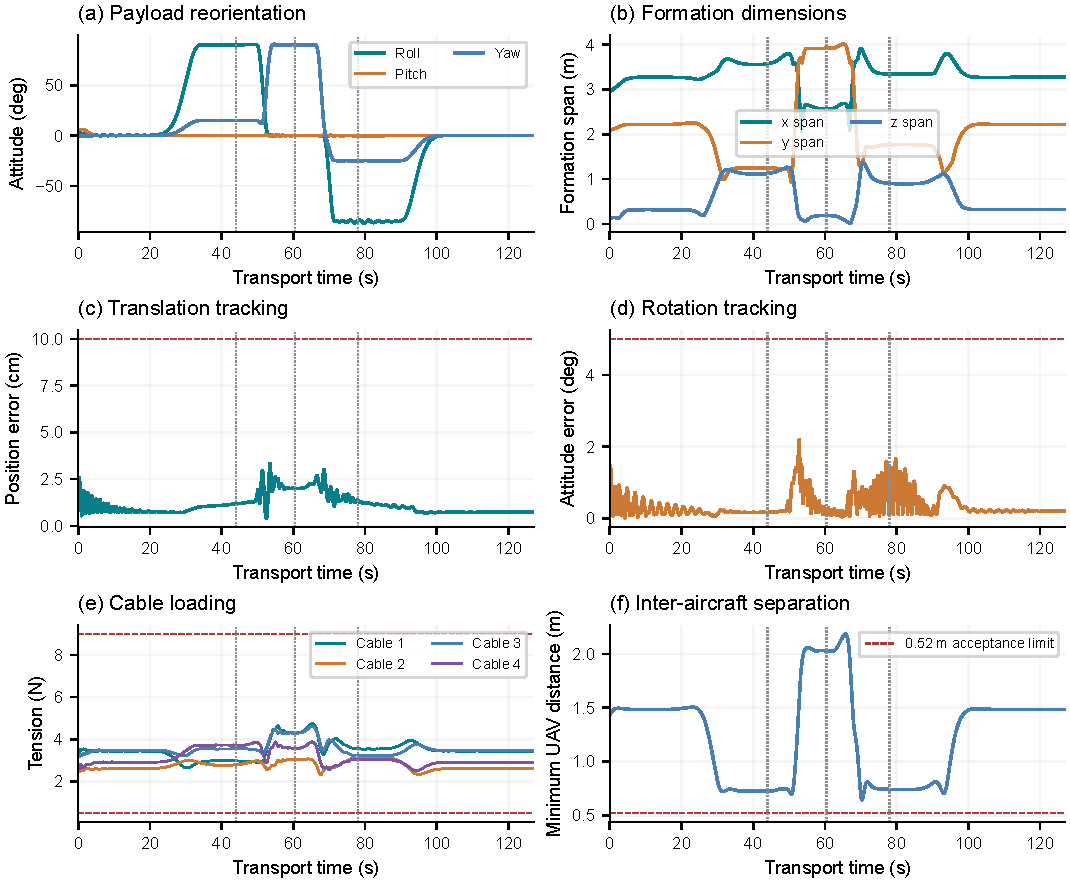
\includegraphics[width=\textwidth]{fig08_course_dynamics.pdf}
\caption{Large-rotation course dynamics. (a) Payload attitude. (b) Aircraft center span along each axis. (c),(d) Position and rotation errors. (e) Cable tensions. (f) Minimum pairwise aircraft center distance. Dotted vertical lines indicate the three payload crossing instants. Dashed horizontal lines indicate the corresponding execution or separation thresholds.}
\label{fig:course_dynamics}
\end{figure*}

\begin{figure*}[!t]
\centering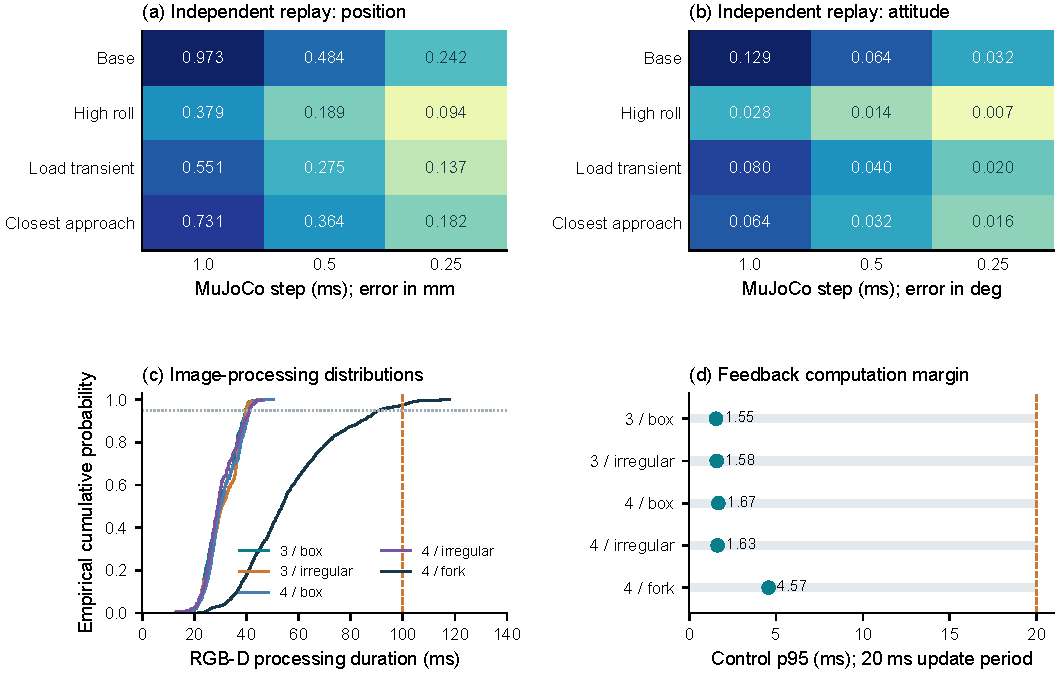
\includegraphics[width=\textwidth]{fig09_validation.pdf}
\caption{Numerical verification and computation distributions. (a),(b) Maximum payload CoM and attitude differences from independent two-second RK4 motor-command replay at three MuJoCo steps, including the base interval and three mechanically demanding course intervals. (c) Empirical cumulative distributions from all archived image-processing durations; the dashed vertical line marks the 100 ms RGB-D request interval. (d) Control-computation p95 values relative to the 20 ms control period. The separate computation paths do not imply 50 Hz image registration or whole-segment replanning.}
\label{fig:validation}
\end{figure*}

\subsection{Computation and numerical cross-checks}
For the four base identified-model configurations, initial whole-segment planning takes 0.74--1.56 s. Image processing p95 is 39.7--41.3 ms, control computation p95 is 1.55--1.67 ms, and sensor age p95 is 120--140 ms. The larger course requires additional conic separation updates and full-surface checks. Its initial plan takes 24.85 s, image processing p95 is 91.03 ms and control computation p95 is 4.57 ms. The observations remain asynchronous, with sensor age p95 of 160 ms. These timings separate pretransport trajectory construction from visual processing and feedback during motion. Force planning uses Clarabel with feasibility tolerance $2\times10^{-8}$, absolute and relative gap tolerances $10^{-7}$, and at most 100 iterations. Moment fitting uses feasibility tolerance $10^{-9}$ and absolute gap tolerance $10^{-10}$. The archived solver diagnostics retain the iteration counts for individual candidates.

Numerical consistency is examined using a two-second interval from the three-aircraft irregular-payload base execution, starting at physical time 29.30 s. A separately coded NumPy rigid-body model integrates the recorded motor inputs with fourth-order Runge--Kutta at 0.25 ms, without resetting the state inside the interval. As the MuJoCo step decreases from 1 to 0.5 and 0.25 ms, the maximum payload CoM difference decreases from 0.973 to 0.484 and 0.242 mm. The corresponding rotation differences are $0.1291^\circ$, $0.0642^\circ$ and $0.0320^\circ$; aircraft CoM differences decrease from 3.468 to 1.727 and 0.862 mm. Figure~\ref{fig:validation}(a),(b) includes this interval together with three additional two-second intervals from the large-angle course: maximum absolute roll, maximum sampled tension variation, and minimum aircraft-envelope clearance. Each interval is replayed continuously without interior state resets. At a 0.5 ms MuJoCo step, the added intervals differ from the independent RK4 replay by at most 0.365 mm in payload CoM and $0.040^\circ$ in attitude; halving the step approximately halves these differences.

A complete closed-loop rerun of that base configuration at a 0.25 ms step also satisfies the execution criteria, with 3.53 cm peak position error, $2.59^\circ$ peak attitude error and 1.20--7.53 N cable tensions. Together, the interval comparison and refined closed-loop execution examine both the numerical force implementation and the resulting feedback trajectory.



\subsection{Implications for cooperative transport}
The experiments connect three different kinds of information. The scan supplies the object's occupied geometry and a consistent frame for calibrated attachments. Tension and motion reveal the mass moments needed to balance and rotate that object. The force-to-endpoint map then converts the identified mechanics into aircraft geometry. The paired base experiment quantifies the effect of supplying those moments, while the sequential-aperture experiment shows how compliant support geometry changes during substantial load rotation.

The evaluated configuration uses calibrated external virtual RGB-D views, static payload mass distributions and known obstacle geometry. These conditions define the sensing and task model of the reported experiments. An onboard implementation introduces camera occlusion, calibration drift and different image coverage; changing payload contents introduces time-varying inertial parameters. These extensions call for corresponding sensing and replanning mechanisms. Within the evaluated setting, the current results establish continuous large-angle closed-loop transport across the specified apertures, with explicit load, cable and aircraft measurements.

\section{Conclusion}
This paper develops a vision- and tension-informed connection between inertial identification and supporting formation geometry for cooperative aerial transport through known obstacles. The payload pose reference family is prescribed; conic optimization selects the cable forces, compliant support endpoints and a feasible timing candidate. A reconstructed surface anchors markerless pose measurements and a nonnegative representation of inertial moments. Integral momentum observations identify the CoM and inertia used by a conic cable-force planner. Compliant endpoint construction and sequential separation then connect these forces to the aircraft formation throughout rotation and aperture passage.

Three-aircraft and four-aircraft rectangular/irregular configurations complete the base task with 2.62--4.10 cm position errors and $0.66$--$2.64^\circ$ attitude errors. The mass-matched five-arm comparison attributes the main base-task tracking gain to CoM correction, while complete-inertia accuracy and transport-only prediction quantify the additional identified moments. A forked payload subsequently completes a 28 m course with successive side-on, horizontal and opposite-side orientations, reaching approximately $\pm90^\circ$ roll while maintaining positive cable tensions and clearance. These findings support the use of identified internal mass moments when coordinating payload attitude and supporting formation through spatial restrictions.

\section*{Funding}
This work was supported in part by the Foundation for Innovative Research Groups of the National Natural Science Foundation of China under Grant 62421004, and in part by the National Natural Science Foundation of China under Grants 62303348 and 62173242.

\section*{Data availability}
The simulation and identification source code, task configurations, true and fitted inertial parameters, archived trajectories, ablation and repeated-seed experiments and figure-generation scripts are available at \url{https://github.com/shepherd-p/ForestSling}. The repository documents the analysis and rerun commands and identifies each experiment by its configuration and random seed. Recorded trajectory visualizations are provided with the reproducibility materials. Proprietary Unreal environment assets are excluded; numerical analysis and MuJoCo simulation do not require those assets.

\begin{thebibliography}{99}
\bibitem{sun2025}
S. Sun, X. Wang, D. Sanalitro, A. Franchi, M. Tognon, J. Alonso-Mora, Agile and cooperative aerial manipulation of a cable-suspended load, Science Robotics 10 (107) (2025) eadu8015. \doi{10.1126/scirobotics.adu8015}.
\bibitem{heins2025}
A. Heins, A. P. Schoellig, Robust Nonprehensile Object Transportation With Uncertain Inertial Parameters, IEEE Robotics and Automation Letters 10 (5) (2025) 4492--4499. \doi{10.1109/LRA.2025.3551067}.
\bibitem{wensing2018}
P. M. Wensing, S. Kim, J. E. Slotine, Linear Matrix Inequalities for Physically Consistent Inertial Parameter Identification: A Statistical Perspective on the Mass Distribution, IEEE Robotics and Automation Letters 3 (1) (2018) 60--67. \doi{10.1109/LRA.2017.2729659}.
\bibitem{petitti2020}
A. Petitti, D. Sanalitro, M. Tognon, A. Milella, J. Cortes, A. Franchi, Inertial Estimation and Energy-Efficient Control of a Cable-suspended Load with a Team of UAVs, 2020 International Conference on Unmanned Aircraft Systems (ICUAS) (2020) 158--165. \doi{10.1109/ICUAS48674.2020.9213842}.
\bibitem{li2021}
G. Li, R. Ge, G. Loianno, Cooperative Transportation of Cable Suspended Payloads With MAVs Using Monocular Vision and Inertial Sensing, IEEE Robotics and Automation Letters 6 (3) (2021) 5316--5323. \doi{10.1109/LRA.2021.3065286}.
\bibitem{nmpc2023}
G. Li, G. Loianno, Nonlinear Model Predictive Control for Cooperative Transportation and Manipulation of Cable Suspended Payloads with Multiple Quadrotors, 2023 IEEE/RSJ International Conference on Intelligent Robots and Systems (IROS) (2023) 5034--5041. \doi{10.1109/IROS55552.2023.10341785}.
\bibitem{pallar2025}
A. Pallar, G. Li, M. Sarvaiya, G. Loianno, Optimal Trajectory Planning for Cooperative Manipulation with Multiple Quadrotors Using Control Barrier Functions, 2025 IEEE International Conference on Robotics and Automation (ICRA) (2025) 2808--2814. \doi{10.1109/ICRA55743.2025.11128734}.
\bibitem{ast2021}
F. Arab, F. A. Shirazi, M. R. H. Yazdi, Planning and distributed control for cooperative transportation of a non-uniform slung-load by multiple quadrotors, Aerospace Science and Technology 117 (2021) 106917. \doi{10.1016/j.ast.2021.106917}.
\bibitem{geng2022}
J. Geng, P. Singla, J. W. Langelaan, Load-Distribution-Based Trajectory Planning and Control for a Multilift System, Journal of Aerospace Information Systems 19 (5) (2022) 366--381. \doi{10.2514/1.I011067}.
\bibitem{lee2010}
T. Lee, M. Leok, N. H. McClamroch, Geometric tracking control of a quadrotor UAV on SE(3), 49th IEEE Conference on Decision and Control (CDC) (2010) 5420--5425. \doi{10.1109/CDC.2010.5717652}.
\bibitem{mujoco2012}
E. Todorov, T. Erez, Y. Tassa, MuJoCo: A physics engine for model-based control, 2012 IEEE/RSJ International Conference on Intelligent Robots and Systems (2012) 5026--5033. \doi{10.1109/IROS.2012.6386109}.
\bibitem{airsim2017}
S. Shah, D. Dey, C. Lovett, A. Kapoor, AirSim: High-Fidelity Visual and Physical Simulation for Autonomous Vehicles, Field and Service Robotics (2017) 621--635. \doi{10.1007/978-3-319-67361-5_40}.
\bibitem{boyd2004}
S. Boyd, L. Vandenberghe, Convex Optimization, Cambridge University Press (2004). \doi{10.1017/CBO9780511804441}.
\bibitem{polyfly2026}
M. Sarvaiya, G. Li, G. Loianno, PolyFly: Polytopic Optimal Planning for Collision-Free Cable-Suspended Aerial Payload Transportation, IEEE Robotics and Automation Letters 11 (3) (2026) 2991--2998. \doi{10.1109/LRA.2026.3655278}.
\bibitem{crazymarl2026}
V. Lorentz, K. Wahba, S. Auddy, M. Toussaint, W. Hönig, CrazyMARL: Decentralized Direct Motor Control Policies for Cooperative Aerial Transport of Cable-Suspended Payloads, 2026 IEEE International Conference on Robotics and Automation (ICRA) (2026) 2013--2020. \doi{10.1109/ICRA57385.2026.11696542}.
\bibitem{icp1992}
P. J. Besl, N. D. McKay, A method for registration of 3-D shapes, IEEE Transactions on Pattern Analysis and Machine Intelligence 14 (2) (1992) 239--256. \doi{10.1109/34.121791}.
\bibitem{chai2026}
Y. Chai, Z. Yang, X. Liang, J. Han, Time-optimal gap-traversal trajectory planning scheme for collaborative aerial transportation systems: An experimental research, Aerospace Science and Technology 169 (2026) 111343. \doi{10.1016/j.ast.2025.111343}.
\bibitem{sunlocal2026}
J. Sun, D. Zhang, Y. Chen, L. Mu, G. Jia, Local obstacle avoidance and trajectory tracking control of multi-quadrotor cooperative transportation system, Aerospace Science and Technology 173 (2026) 111670. \doi{10.1016/j.ast.2026.111670}.
\bibitem{chan2026}
Y. Y. Chan, Y. Shu, W.-H. Chen, K. K. H. Ng, Time-optimal motion planning of cable-suspended payload quadcopters using spatial reformulation, Aerospace Science and Technology 169 (2026) 111460. \doi{10.1016/j.ast.2025.111460}.
\end{thebibliography}

\end{document}
